\section{Introduction}

Social media posts are often useful to detect real-time adverse drug reactions (ADR) compared to other available resources such as clinical reports, health records. They can be a valuable tool for pharmaceutical companies to obtain feedback about medication~\cite{plachouras2016quantifying, huynh2016adverse}. Vast number of tweets mentioned in drug names and adverse drug re-actions can easily be collected in real-time. Plachouras et al.~\cite{plachouras2016quantifying} reported that from July 9 to September 4, 2014 (shown in figure~\ref{fig:daily-tweets-adr}), on average 179K tweets were mentioning drug names and 721 tweets were containing ADRs. They proposed an ecosystem on clinical reports and social media posts can be useful to pharmaceutical companies - shown in figure~\ref{fig:ecosystem-pharmaceutical}.

\begin{figure}[h]
	\centering
	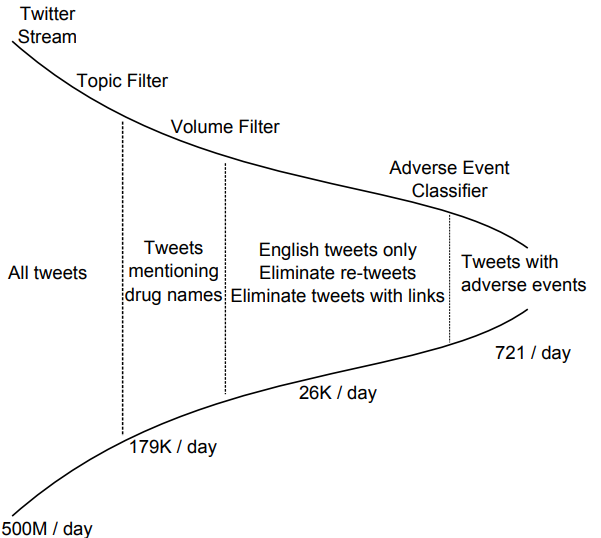
\includegraphics[width=0.99\linewidth]{Figures/g.png}
	\caption{Avg. daily tweets containing ADR from July 9 to September 4, 2014 by Plachouras et al.~\cite{plachouras2016quantifying}}
	\label{fig:daily-tweets-adr}
\end{figure}

\begin{figure}[h]
	\centering
	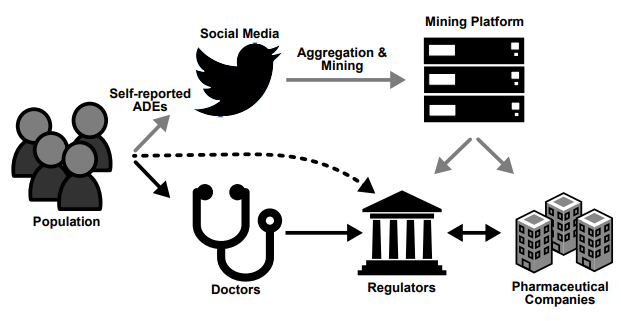
\includegraphics[width=0.99\linewidth]{Figures/j.png}
	\caption{The ecosystem of pharmaceutical companies, regulators, doctors, patients and social media Plachouras et al.~\cite{plachouras2016quantifying}.}
	\label{fig:ecosystem-pharmaceutical}
\end{figure}

The problem of detecting drug names and adverse drug reactions mentioning social media, especially in tweets has been extensively studied in recent years~\cite{weissenbacher2018overview}. Denecke et al.~\cite{DENECKE20091870} performed a content analysis of medical social media data, in particular question \& answer portals, weblogs, reviews, and wikis. The researchers have essentially framed the task of medication name extraction and ADR detection as a binary classification problem. Machine learning techniques are widely used in this task. Deep learning techniques are becoming popular of late. In this paper, we will give short reviews of techniques used by various researchers. 

The review is divided into a couple of sections: preprocessing, model, annotation, evaluation, conclusion.